\documentclass[10pt,a4paper,titlepage]{report}
\usepackage[utf8]{inputenc}
\usepackage[francais]{babel}
\usepackage[T1]{fontenc}
\usepackage{amsmath}
\usepackage{amsfonts}
\usepackage{amssymb}
\usepackage{graphicx}
\usepackage{hyperref}
\author{MONGODIN Maxime; HIRACLIDES Nicolas;\\
 LESIEUR Christophe; KOWALEWSKI Matthieu}
\title{Rapport de Génie Logiciel 2}
\begin{document}
\maketitle
\tableofcontents
\newpage
\chapter*{Introduction}
\addcontentsline{toc}{chapter}{Introduction}
Dans le cadre de l'école virtuelle de L'EISTI nommée AREL, l'école a besoin de gérer un certain nombre de questionnaires. L'objectif du premier projet génie logiciel était d'établir l'ensemble de la base de données permettant de gérer les données générées par ces questionnaires.


Dans ce deuxième projet génie logiciel, nous devons concevoir un logiciel permettant de gérer et de traiter des QCM. En d’autres termes, nous devons développer une interface capable de créer des QCM, d’y répondre et de stocker et exploiter ces données.
Il nous faudra pour cela planifier le projet dans son intégralité en respectant le temps qui nous a été imparti.

\newpage
\chapter{Présentation du projet}

	\section{Expression des besoins}
		Notre logiciel doit pouvoir gérer trois types d’utilisateurs : enseignants, élèves et administrateurs.
		
		
		Les administrateurs  ont comme fonction de  :
		\begin{itemize}
			\item définir d’autres utilisateurs quel que soit leur rôle. Pour un professeur ils préciseront le domaine d’enseignement.

			\item définir une promotion (liste d’élèves).

			\item définir et modifier les modules enseignés à l’école en prenant en compte le nom du module, les modules prérequis et le syllabus du module.
		\end{itemize}
		
		

	Les professeurs doivent pouvoir :
	\begin{itemize}
			\item définir un QCM qui comprend des questions, des réponses prédéfinies (au moins deux par question) vraies ou fausses.

			\item chaque QCM peut être privé ou public. C’est-à-dire qu’un QCM privé n’est utilisable que par le professeur qui l’a créé. Le rendre public, le rend utilisable par tous les professeurs.
			\item créer une session de QCM avec dates de début et de fin, associée à un module et une promotion. On peut répondre à un QCM plusieurs fois seulement si cela est précisé par le professeur.

			\item consulter les résultats complets ou partiels des QCM à tout moment soit par élève, soit sous forme de statistiques (écart type, moyenne, …)

	\end{itemize}
	
	

Les élèves quant à eux peuvent :
\begin{itemize}
	\item répondre à un QCM dans lequel il est inscrit entre les dates de début et fin du QCM et voir un message d’avertissement en dehors de ces dates.
	\item consulter les résultats d’un QCM auquel il a participé une fois que la session est fermée.

\end{itemize}

	\section{Contrainte Plateforme}
		Pour ce projet, nous avons comme contrainte d'implémenter le code sous Java version 1.7. 
		Nous devons aussi utiliser comme méthode d'analyse et de conception l'UML avec la persistance des données. 
Nous utiliserons StarUML afin de réaliser les différents diagrammes. 
Les objets doivent communiquer entre eux à travers des interfaces. 
la sauvegarde des données à la fin du programme ou sur commande pour les données modifiées uniquement est obligatoire.

	\section{Ressources Humaines}
	Notre équipe se compose de quatre membres qui sont les suivants :
	\begin{itemize}
		\item	MONGODIN Maxime
			\begin{itemize}
			 \item[•] Etudiant à l’EISTI de Cergy
			 \item[•] connaissance informatique : C, C++, langage web, Ocaml, Pascal, Java. 

			\end{itemize}
		

		\item	KOWALEWSKI Matthieu
			\begin{itemize}
			 \item[•] Etudiant à l’EISTI de Cergy
			 \item[•] connaissance informatique : C, langage web, Ocaml, Pascal, Java. 

			\end{itemize}
	\item	HIRACLIDES Nicolas
			\begin{itemize}
			 \item[•] Etudiant à l’EISTI de Cergy
			 \item[•] connaissance informatique : C, langage web, Ocaml, Pascal, Java. 

			\end{itemize}
		\item	LESIEUR Christophe
			\begin{itemize}
			 \item[•] Etudiant à l’EISTI de Cergy
			 \item[•] connaissance informatique : C, langage web, Ocaml, Pascal, Java. 

			\end{itemize}
	\end{itemize}
	\section{Planning}
	Nous avons décidé d'attribuer à chaque membre de l'équipe une partie du projet qu'il devrait analyser, conceptualiser et implémenter du début à la fin du projet. Les découpages actuelles des tâches vont sans doute évoluer en fonction du temps et de l'avancement du projet, ainsi que pour respecter l'équité de la quantité de travail à fournir par chaque membre.
	Voici donc notre diagramme de Gantt :
	\begin{figure}[h!]
\caption{Diagramme de Gantt}
\centering
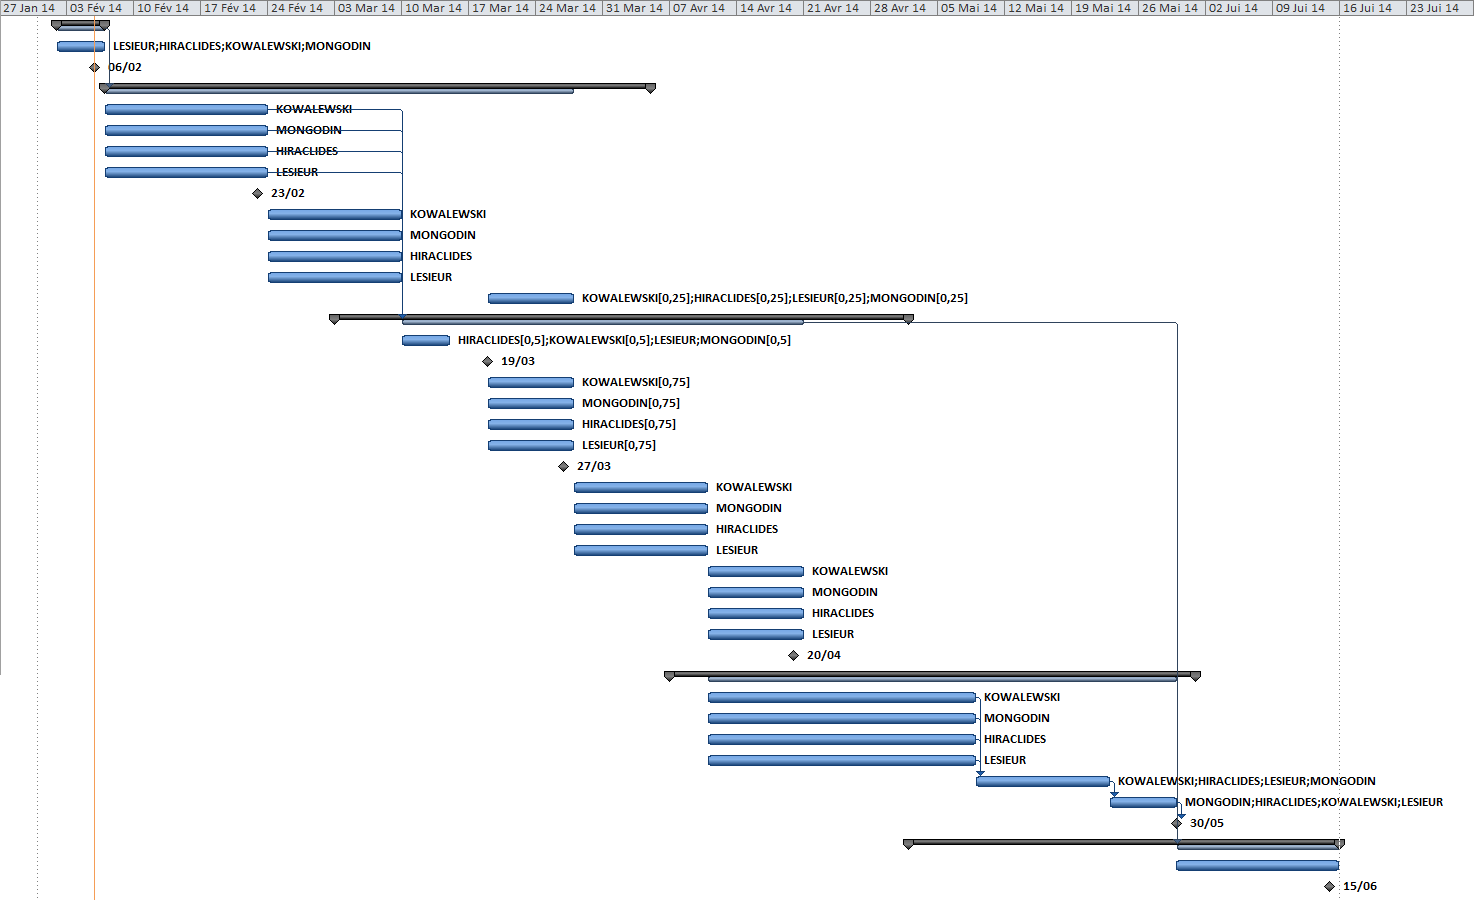
\includegraphics[scale=0.3]{Include/gantt.png}
\end{figure}
\newpage
Les différentes parties du diagramme sont détaillées ici :
	\begin{figure}[h!]
\caption{Cahier Des charges}
\centering
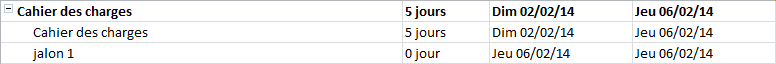
\includegraphics[scale=0.6]{Include/cahier.png}
\end{figure}
	\begin{figure}[h!]
\caption{Analyse}
\centering
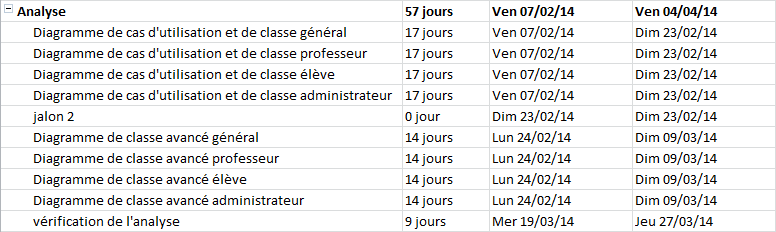
\includegraphics[scale=0.6]{Include/Analyse.png}
\end{figure}
	\begin{figure}[h!]
\caption{Conception}
\centering
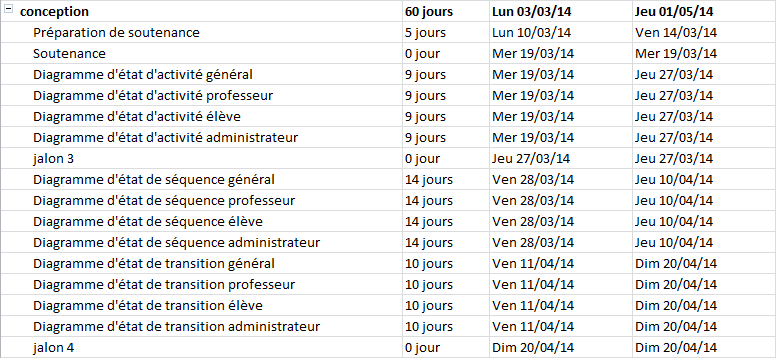
\includegraphics[scale=0.6]{Include/Conception.png}
\end{figure}
	\begin{figure}[h!]
\caption{Implémentation}
\centering
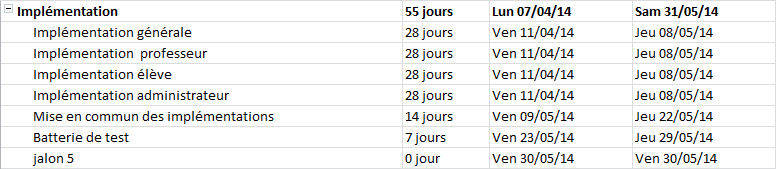
\includegraphics[scale=0.6]{Include/Implementation.png}
\end{figure}
	\begin{figure}[h!]
\caption{Synthèse}
\centering
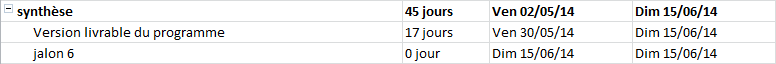
\includegraphics[scale=0.6]{Include/Synthese.png}
\end{figure}
\newpage
\chapter{Analyse}
\section{Cas d'utilisation}
	Nous avons modélisé le projet sous forme de différents diagrammes de cas d'utilisation afin de pouvoir définir l'ensemble des différents besoins que nous devons réaliser pour ce projet.
	\subsection{Diagramme Général}
		Le premier diagramme est un diagramme plutôt général, il est peu détailler mais reprend globalement les différentes fonctionnalités demandées.
		\begin{figure}[h!]
		\caption{Diagramme Général}
		\centering
		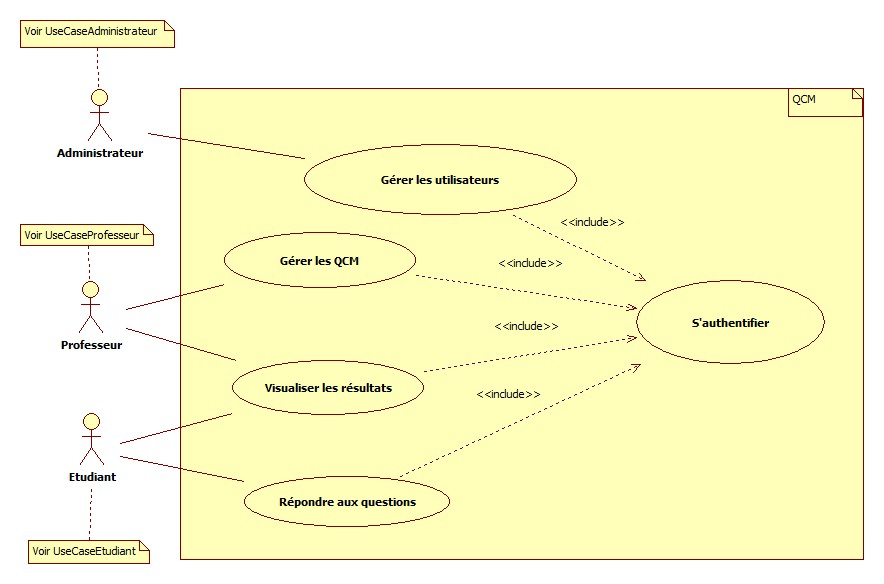
\includegraphics[scale=0.4]{Include/General.jpg}
\end{figure}
\newline
	\begin{tabular}{|c|p{8cm}|}
	\hline 
	\multicolumn{2}{|c|}{\textbf{Fiche de descriptive : s'authentifier}} \\ 
	\hline 
	\textbf{Description} & Tous les utilisateurs doivent se connecter  avant de réaliser les différentes actions qui leur sont attribuées \\  
	\hline
	\textbf{Règle d'initiation} & Les utilisateurs doivent déjà avoir un compte d'authentification créé par un administrateur \\ 
	\hline 
	\textbf{Règle de terminaison} & L'authentification se déconnecte à la fin de l'utilisation du logiciel ou à la déconnexion de ce dernier. \\ 
	\hline 
	\textbf{Règle d'exception} & Aucune \\ 
	\hline 
	\textbf{Relation} & Il s'agit d'un prérequis pour accéder à n'importe quelles autres fonctionnalités.\\ 
	\hline 
	\end{tabular} \newline\newline
	Les différents cas d'utilisations présentés sur le diagramme sont expliqués plus en détails par la suite.
	
	
	\subsection{Diagramme de cas d'utilisation pour les administrateurs}
	Ce diagramme est en rapport avec les administrateurs.
	\begin{figure}[h!]
		\caption{Diagramme Administrateur}
		\centering
		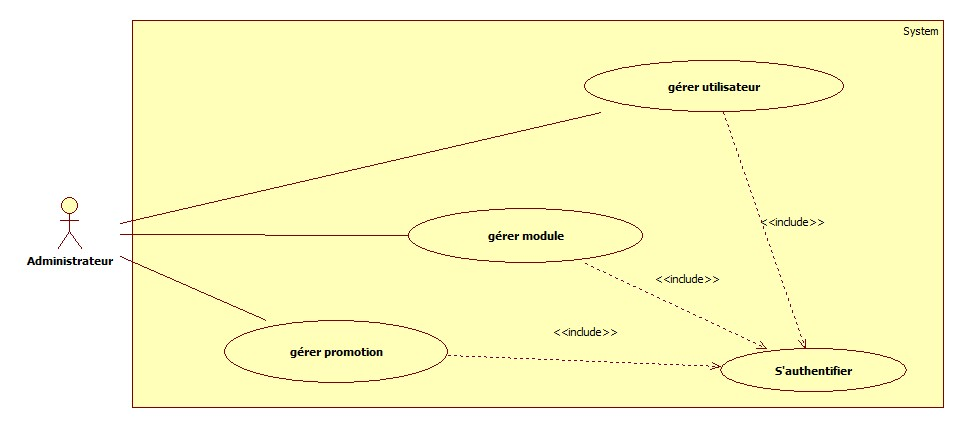
\includegraphics[scale=0.4]{Include/admin.jpg}
\end{figure}

	\begin{tabular}{|c|p{8cm}|}
	\hline 
	\multicolumn{2}{|c|}{\textbf{Fiche de descriptive : Gérer utilisateurs}} \\ 
	\hline 
	\textbf{Description} & L'administrateur doit pouvoir, via une autentification, créer un utilisateur \\  
	\hline
	\textbf{Règle d'initiation} & L'administrateur doit avoir son nom d'utilisateur et son mot de passe valide pour s'authentifier.
				L'utilisateur créé ne doit pas déjà exister. \\ 
	\hline 
	\textbf{Règle de terminaison} & Création d'un utilisateur dans la base de données. \\ 
	\hline 
	\textbf{Règle d'exception} & Aucune \\ 
	\hline 
	\textbf{Relation} & Ce cas inclus le cas s'autentifier
				Ce cas peut entrainer la précision du domaine d'enseignement dans le cas où un professeur est défini
 \\ 
	\hline 
	\end{tabular}
	
		\begin{tabular}{|c|p{8cm}|}
	\hline 
	\multicolumn{2}{|c|}{\textbf{Fiche de descriptive : Gérer module}} \\ 
	\hline 
	\textbf{Description} & L'administrateur doit pouvoir, via une autentification, créer un module \\  
	\hline
	\textbf{Règle d'initiation} & Le module créé ne doit pas déjà exister.
                Le module désigné comme prérequis doit exister.
                Pour modifier un module, ce dernier doit exister. \\ 
	\hline 
	\textbf{Règle de terminaison} & Création d'un module dans la base de données. \\ 
	\hline 
	\textbf{Règle d'exception} & Aucune \\ 
	\hline 
	\textbf{Relation} & Ce cas inclus le cas s'autentifier
				Ce cas peut entrainer la précision des modules prérequis
 \\ 
	\hline 
	\end{tabular}\newline \newline \newline
	\begin{tabular}{|c|p{8cm}|}
	\hline 
	\multicolumn{2}{|c|}{\textbf{Fiche de descriptive : Gérer promotion}} \\ 
	\hline 
	\textbf{Description} & L'administrateur doit pouvoir, via une autentification, créer une promotion \\  
	\hline
	\textbf{Règle d'initiation} &  La promotion créée ne doit pas déjà exister.
                Les élèves d'une promotion doivent exister. \\ 
	\hline 
	\textbf{Règle de terminaison} & Création d'une promotion dans la base de données. \\ 
	\hline 
	\textbf{Règle d'exception} & Aucune \\ 
	\hline 
	\textbf{Relation} & Ce cas inclus le cas s'autentifier
 \\ 
	\hline 
	\end{tabular} \\  
	\newpage
	\subsection{Diagramme de cas d'utilisation pour les professeurs}
	Ce diagramme est en rapport avec les professeurs.
	\begin{figure}[h!]
		\caption{Diagramme Professeur}
		\centering
		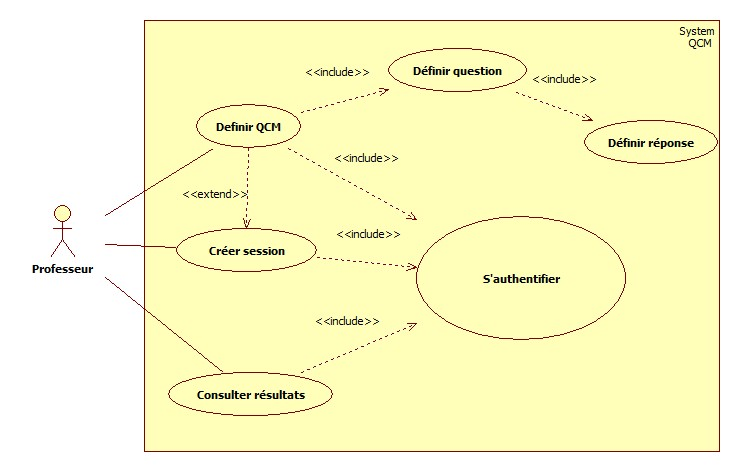
\includegraphics[scale=0.5]{Include/Professeur.jpg}
\end{figure}

	
	\begin{tabular}{|c|p{8cm}|}
	\hline 
	\multicolumn{2}{|c|}{\textbf{Fiche de descriptive : Définir QCM}} \\ 
	\hline 
	\textbf{Description} &Création d'un ensemble de questions, elles-mêmes munies
	de plusieurs réponses fermées 
	(qualitative nominale), et qui sont définies commes vraies ou fausses. Lors de la
	création du QCM,
 le professeur précise s'il est privé (seul le créateur peut l'utiliser)
	ou public (d'autres professeurs peuvent l'utiliser). Un libellé doit aussi être donné
	pour identifier ledit QCM.
 \\  
	\hline
	\textbf{Règle d'initiation} & Le professeur est authentifié et choisit de créer un QCM.

	Une QCM possédant le même libellé ne doit pas déjà exister.

	Une QCM doit être composé d'au moins 1 question.

	Une question doit avoir au moins 2 réponses.
	Une réponse est soit vraie, soit fausse.


 \\ 
	\hline 
	\textbf{Règle de terminaison} & Un objet QCM est créé.
	Le libellé est disponible dans la liste des QCMs disponible lors d'une session.
	Invite de création de session pour le QCM créé.
	 \\ 
	\hline 
	\textbf{Règle d'exception} & Aucune \\ 
	\hline 
	\textbf{Relation} & Le cas d'usage 'S'authentifier' est inclus dans le cas d'usage 'Définir QCM' car il 
	permet au professeur de s'authentifier.

	Les cas d'usage 'Définir question' et, par extension, 'Définir réponse', sont inclus
	dans 'Définir QCM' car ils sont des étapes nécessaires à la création d'un QCM.
 \\ 
	\hline 
	\end{tabular} 
	\newline
	\newline
\begin{tabular}{|c|p{8cm}|}
	\hline 
	\multicolumn{2}{|c|}{\textbf{Fiche de descriptive: Créer Session}} \\ 
	\hline 
	\textbf{Description} & Création d'une session de QCM donné, limitée dans le temps par une date de début et
	une date de fin, toute deux précisées par le professeur. Cette session est associée 
	à une promotion, pour savoir quels élèves doivent passer le QCM; un module, pour 
	savoir dans le cadre de quel enseignement ces élèves sont interrogés. Un nombre de 
	répétitions (par défaut, 1) est aussi indiqué, pour donner le nombre maximum de fois
	où un élève donné a le droit de répondre au QCM.
 \\  
	\hline
	\textbf{Règle d'initiation} & Le professeur doit être authentifié.
	Le QCM indiqué doit exister.
	La promotion doit exister et être non vide.
	Le module doit exister.
	La date de début doit être avant la date de fin.
	Un nombre de répétitions est attendu. \\ 
	\hline 
	\textbf{Règle de terminaison} & Création d'un objet session.
	Création d'un objet résultats, associé à la session créée, qui stockera les réponses
	données par chaque élève lors de cette session.
 \\ 
	\hline 
	\textbf{Règle d'exception} & 
	Si le QCM indiqué n'existe pas, alors le professeur peut choisir d'en créer un.
	La date de début peut être la même que celle de fin : la session dure alors une
	unique journée.
	Si le aucune nombre de répétitions n'est précisé, celui-ci est fixé par défaut à 1.
 \\ 
	\hline 
	\textbf{Relation} & Le cas d'usage 'S'authentifier' est inclus dans le cas d'usage 'Séfinir session' car il 
	permet au professeur de s'authentifier.
	Le cas d'usage 'Définir QCM' est une extension de 'Définir session', car il peut être appelé
	au cours de celui-ci.
 \\ 
	\hline 
	\end{tabular} 	\newline
	\newline
	
	
	\begin{tabular}{|c|p{8cm}|}
	\hline 
	\multicolumn{2}{|c|}{\textbf{Fiche de descriptive : Consulter les résultats}} \\ 
	\hline 
	\textbf{Description} & Un professeur doit pouvoir consulter les résultats des sessions qu'il a créées. Ceux-ci
	peuvent être définitifs (session terminée), ou bien partiels (session toujours en cours).
	Deux types de résultats peuvent alors être visualisés : pour chaque élève, ses réponses
	ainsi que son score final, ou bien les statistiques de l'ensemble des élèves, à savoir la
	moyenne et l'écart-type de tous les scores, et la fréquence de bonnes réponses par
	question. \\  
	\hline
	\textbf{Règle d'initiation} & Le professeur doit être authentifié.
	Le professeur voulant consulter les résultats d'une session doit être le créateur de cette
	session.
	La session doit avoir commencé (des résultats doivent être enregistrés pour être visualisés).
		
 \\ 
	\hline 
	\textbf{Règle de terminaison} & Aucune \\ 
	\hline 
	\textbf{Règle d'exception} & Si la session n'a pas encore commencé, un message affiche cet état de fait et invite le
	professeur à retenter le jour de début de session.
 \\ 
	\hline 
	\textbf{Relation} & 
	Le cas d'usage 'S'authentifier' est inclus dans le cas d'usage 'Consulter résultats' car il 
	permet au professeur de s'authentifier. \\ 
	\hline 
	\end{tabular} 
	\subsection{Diagramme de cas d'utilisation pour les étudiants}
	Ce diagramme est en rapport avec les étudiants.
	\begin{figure}[h!]
		\caption{Diagramme Etudiant}
		\centering
		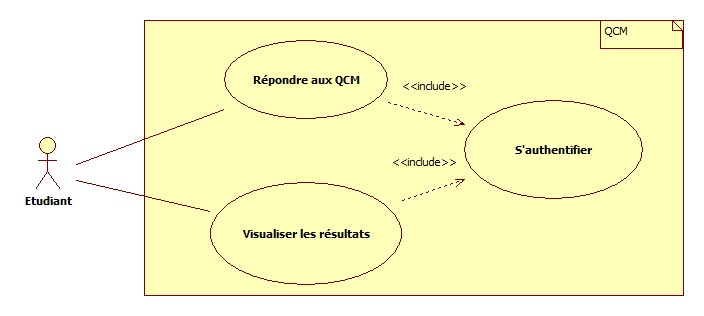
\includegraphics[scale=0.4]{Include/Etudiant.jpg}
\end{figure}

	\begin{tabular}{|c|p{8cm}|}
	\hline 
	\multicolumn{2}{|c|}{\textbf{Fiche de descriptive : Répondre aux QCM}} \\ 
	\hline 
	\textbf{Description} & L'étudiant peut, via une authentification, répondre à des QCM. \\  
	\hline
	\textbf{Règle d'initiation} & L'étudiant doit être dans la promotion qui répond à ce QCM et il doit se connecter durant la session. \\ 
	\hline 
	\textbf{Règle de terminaison} & Une fois que l’étudiant à répondu à un QCM, on doit noter l'étudiant comme ayant validé ce QCM, récupérer les réponses données et les stocker. \\ 
	\hline 
	\textbf{Règle d'exception} & Affichage d’un message d'erreur si l'étudiant essaye de répondre aux QCM en dehors des dates de début et de fin du QCM \\ 
	\hline 
	\textbf{Relation} & Répondre aux QCM nécessite de s'authentifier \\ 
	\hline 
	\end{tabular} 
	\newline \newline
	\newline
		\begin{tabular}{|c|p{8cm}|}
	\hline 
	\multicolumn{2}{|c|}{\textbf{Fiche de descriptive : Visualiser les résultats}} \\ 
	\hline 
	\textbf{Description} & L'étudiant peut, via une authentification, visualiser ses résultats. \\  
	\hline
	\textbf{Règle d'initiation} & L’étudiant doit avoir répondu aux QCM, doit se connecter une fois la session terminée, et il ne doit pas pouvoir visualiser les QCM auquel il n’a pas répondu. \\ 
	\hline 
	\textbf{Règle de terminaison} & Aucune \\ 
	\hline 
	\textbf{Règle d'exception} & Aucune \\ 
	\hline 
	\textbf{Relation} & Visualiser les résultats nécessite de s'authentifier \\ 
	\hline 
	\end{tabular} 
\section{Diagrammes de classe}
Le diagramme de classes est un schéma utilisé en génie logiciel pour présenter les classes et les interfaces des systèmes ainsi que les différentes relations entre celles-ci. Ce diagramme fait partie de la partie statique d'UML car il fait abstraction des aspects temporels et dynamiques.
\subsection{Diagramme de classe général}
Dans un premier temps nous nous intéressons à la super classe Utilisateur dont un certain nombre de propriétés va engendrer des attributs pour les différents utilisateurs du logiciel.
Chacun des utilisateurs est détaillé dans la suite du rapport.
\begin{figure}[h!]
		\caption{Diagramme Administrateur}
		\centering
		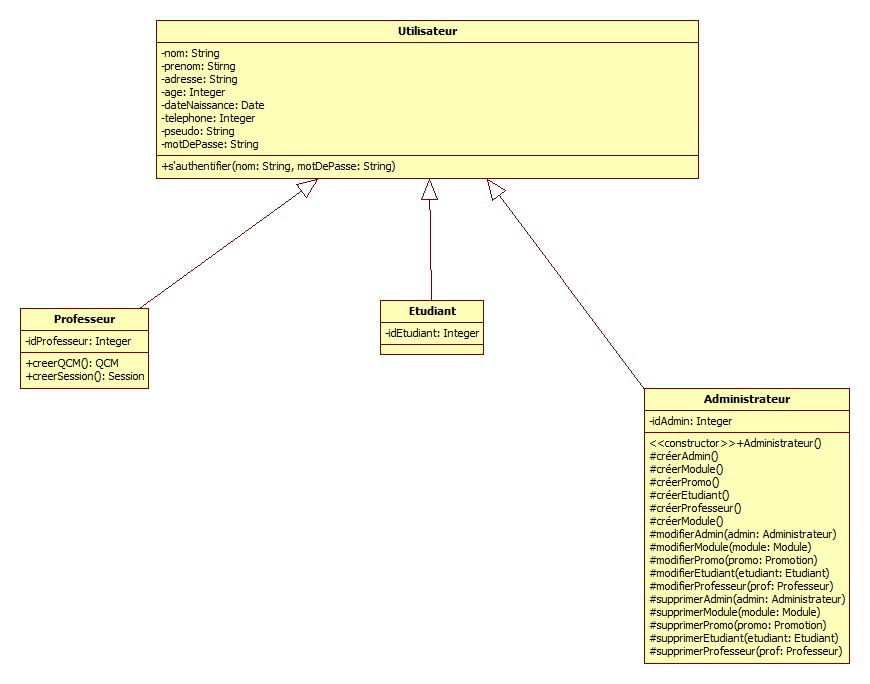
\includegraphics[scale=0.4]{Include/classe/General.jpg}
\end{figure}\newpage
\subsection{Diagramme de classe relatif aux administrateurs}
Les administrateurs peuvent créer, modifier ou même supprimer un certain nombre d'éléments dans le logiciel. Un premier administrateur devra être ajouter manuellement afin de pouvoir générer un ensemble d'utilisateurs et de QCM.
\begin{figure}[h!]
		\caption{Diagramme Administrateur}
		\centering
		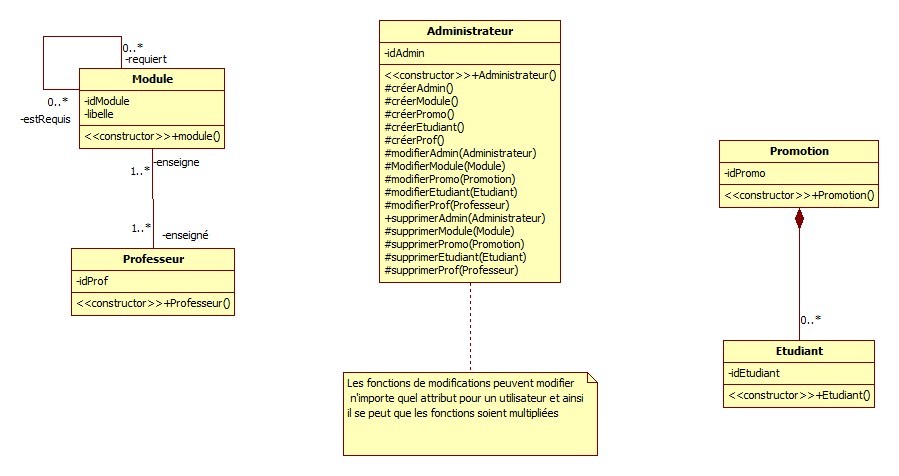
\includegraphics[scale=0.4]{Include/classe/Administrateur.jpg}
\end{figure}
\subsection{Diagramme de classe relatif aux professeurs}
Le professeur peut créer un QCM ainsi que la session associée à ce QCM. On y retrouve ici un lien avec l'étudiant qui est détaillé dans le prochain diagramme.
\begin{figure}[h!]
		\caption{Diagramme Professeur}
		\centering
		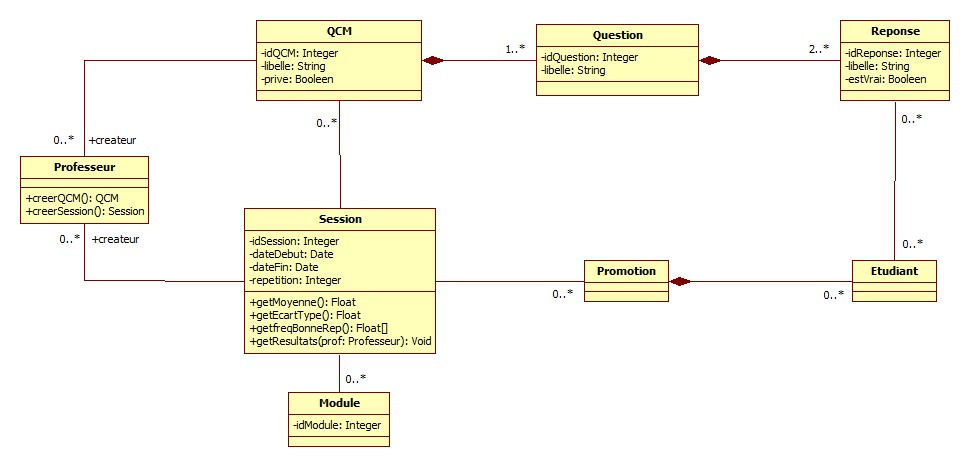
\includegraphics[scale=0.4]{Include/classe/prof.jpg}
\end{figure}\newpage
\subsection{Diagramme de classe relatif aux étudiants}
L'étudiant va pouvoir répondre aux questions d'un ou plusieurs QCM dans la limite ou la session est encore active. Si la session est terminée l'étudiant peut alors visualiser ses résultats.
\begin{figure}[h!]
		\caption{Diagramme Etudiant}
		\centering
		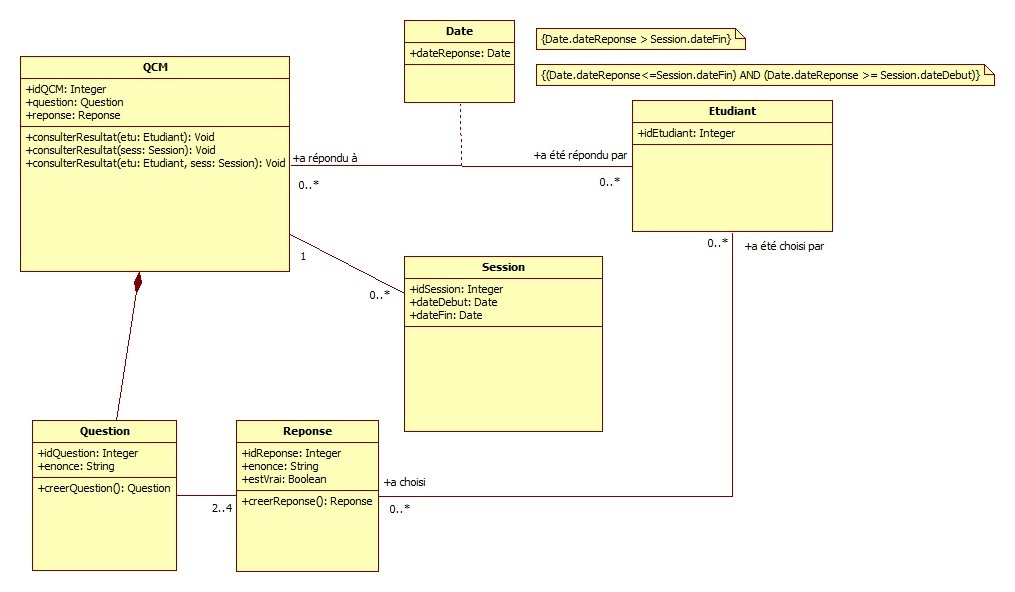
\includegraphics[scale=0.5]{Include/classe/etudiant.jpg}
\end{figure}

\chapter*{Conclusion}
\addcontentsline{toc}{chapter}{Conclusion}
Pour conclure, ce livrable contient une partie de l'analyse du projet. Il va être modifier dans les semaines qui suivent pour être beaucoup plus précis et ainsi mieux cerner le problème initial.
Les diagramme proposées ne sont pas définitif ils pourront être modifiés tout au long des prochains livrables.

\end{document}